\documentclass[10pt,conference,compsocconf]{IEEEtran}

%\usepackage{times}
%\usepackage{balance}
\usepackage{amsmath}
\usepackage{url}
\usepackage{graphicx}
\usepackage[pdftex]{hyperref}
\usepackage[utf8]{inputenc}

\begin{document}
\title{Inpainting with controlled dimensionality reduction in the Fourier domain}

\author{
  Patrick Bänziger, Kaspar Etter, Jan Rüegg\\
  Department of Computer Science, ETH Zurich, Switzerland
}

\maketitle

\begin{abstract}
  This paper suggests a novel approach to restore noisy images.
  ((( TODO )))
  The abstract should really be written last, along with the title of
the paper. The four points that should be covered:
\begin{enumerate}
\item State the problem.
\item Say why it is an interesting problem.
\item Say what your solution achieves. (CLAIM!)
\item Say what follows from your solution.
\end{enumerate}
\end{abstract}

\section{Introduction}
Inpainting is about reconstructing the missing spots of an image by guessing the correct values. The quality of such a restoration method can be evaluated by masking an image and comparing the result with the original.\\
Our approach is based on the assumption that (natural) images have some underlying characteristic that can be distinguished from noise. The computed pixels can be viewed as a disturbed version of the genuine ones, hence the goal is to get rid of this noise. We do so by analyzing image patches in the Fourier space, removing the weak frequencies that (hopefully) capture the noise and thereby recovering the intrinsic signal.\\
We repeat this procedure with the newly determined values until the error of a randomly chosen validation set converges or the maximum number of iterations is reached. For a faster start, we initialize our reconstructed image with what we call Gaussian interpolation: Using MATLAB's filtering function, we compute a weighted sum over all the neighboring pixels that are known. In order to determine the best threshold for suppressing weaker frequencies, we randomly remove even more pixels from the image and use them as a validation set (for which we know the correct values).

\section{Methods}
\subsection{Related work}
Without actually knowing the broad field of research about inpainting (also known as image interpolation), we could not find any papers covering similar concepts as ours. Most methods are based on partial differential equations or some form of texture synthesis.

\subsection{New approach}
As outlined in the introduction, we combined several ideas for obtaining an inpainting algorithm that provides both good results and fast performance. The input of our algorithm is the image to be restored together with a mask that indicates its unknown spots.\\
Before entering the iterative part of our algorithm, the following three steps are performed (as seen in figure ??):
\begin{enumerate}
\item In order to guide the elimination of frequencies by finding the optimal threshold (as described below), we first remove additional pixels from the image and use them as the validation set. The fraction of additional pixels to be removed is a global parameter, which we optimized using gradient descent (as explained in section ??).
\item Since our reduction in the Fourier space works best with framed patches, we frame the complete image by mirroring its margin. (The size of the frame is another optimizable global parameter.)
\item ...
\end{enumerate}


---------------------------\\


We use an iterative scheme to determine the right parameters used in our algorithm. For this, we use cross-validation: We randomly remove a percentage of pixels from the image as a validation set. (((STILL VALID?))) We then use this set to test the accuracy of our parameters and determine the best set of parameters for this image.

We then proceed to the main steps of the algorithm:
\begin{enumerate}
\label{algo}
\item \label{algo:step1}
We use a Gaussian to interpolate the missing pixels indicated by the mask, using a convolution operation. Both $\sigma$ and the size of the Gaussian matrix are determined by the cross-validation. (((TODO?!)))
This step is required by the Fourier transform which cannot ignore samples. (((Humm)))

\item \label{algo:step2}
We transform the image to the Fourier domain. In this domain we set the magnitudes of all frequencies to zero which are below the $n$-th percentile threshold. Again, our ideal cutoff $n$ is determined by cross-validation using a loop.

\item \label{algo:step3}
In this last step, we invert the Fourier transform and combine the reconstructed image with the undamaged part of the image, yielding our result.

\end{enumerate}

In our implementation, we use several tweaks to improve performance or quality:
\begin{itemize}
\item We perform the Fourier transform and thresholding on image patches to allow an individual threshold per patch.
\item To avoid discontinuity (Image \ref{fig:boundaryArtifacts}) at the boundary of the patches, we use a frame around the actual patch to capture more information. (Image \ref{fig:framing}) This frame is not filled in by the reconstructed patch from the Fourier step. The frames of adjacent patches are overlapping if the frame size is set to a value larger than zero. At the image boundaries, we replicate the outermost pixels to provide a sufficient frame.\end{itemize}
((( TODO )))
Describe your idea and how it was implemented to solve
  the problem. Survey the related work, giving credit where credit is
  due. 
  
  The style in this section should read as if you were verbally
describing the conduct of the experiment. 
The methods section is not a step-by-step, directive,
protocol as you might see in your lab manual, but detailed enough such
that an interested reader can reproduce your
work.
The methods
section should describe what was
done to answer the research question, describe how it was done,
justify the experimental design, and
explain how the results were analyzed.

The methods section of a research paper provides the information by
which a study's validity is judged.
Therefore, it requires a clear and precise description of how an
experiment was done, and the rationale
for why specific experimental procedures were chosen.
It is usually helpful to
structure the methods section by:
\begin{enumerate}
\item Describing the algorithms used in the study, briefly including
  details such as hyperparameter values (e.g. thresholds), and
  preprocessing steps (e.g. normalizing the data to have mean value of
  zero).
\item Explaining how the materials were prepared, for example the
  images used and their resolution.
\item Describing the research protocol, for example which examples
  were used for estimating the parameters (training) and which were
  used for computing performance.
\item Explaining how measurements were made and what
  calculations were performed. Do not reproduce the full source code in
  the paper, but explain the key steps.
\end{enumerate}

\subsection{Online threshold estimation}
In the algorithm as described above, we have many different parameters that are required to be tuned

\subsection{Offline parameter estimation}
As shown in table \ref{parameters}, there are a total of 10 parameters in our algorithm that can be set.
For many of them, it is quite clear what values should be used. For example, the size of the gauss kernel
should be a bit larger than the biggest assumed hole in the image. For others, like the maximum number of
iterations, it is not so clear. And yet others have a clear speed / accuracy tradeoff, like the stopping
conditions of the online threshold estimation.

Because we thought it not feasable to tune all the parameters by hand, we wrote an algorithm to
do the offline parameter estimation. The idea is to do this once for a few representative images, and get
parameters that can model as closely as possible many of the images we are interested in.
Our proposed method combines a gradient descent method with ideas from cross-validation, and tunes our
10-dimensional parameter-space, maximising time and accuracy.

\subsubsection{Error function}
When doing a minimization of any kind, an error function is needed. Of course we already had the error function
of the evaluation script, that gives a mean over the squared differences of the reconstructed to the original
image. However, using only an error measure, the time would potentially grow to infinity to get the best accuracy possible during tuning.

Therefore we tried different error function including both, the image error $E$, and the time $T$ spent (see table \ref{error_function_table}). The image error here is the average
squared error of a reconstructed pixel to the original pixel, scaled with a factor (usually about 10000), while the time is measured in seconds.

\begin{table*}
  \centering
  \begin{tabular}{|l|p{5cm}|p{5cm}|}
    \hline
    Function&Advantages&Disadvantages\\
    \hline
    $\exp(E)+\exp(T)$ & Increases cost fast to avoid $E$ or $T$ over a certain threshold & Not enough gradient for very low $E$, $T$ values\\
    \hline
    $(1-\exp(E))*(1-\exp(T))$ & Makes it possible to have large times for very low errors & Works also the other way around, and optimization only minimizes time\\
    \hline
    $E + T$ & Everywhere a good gradient & Time from 60 to 59 seconds is same \textit{improvement} as time from 2 to 1 second\\
    \hline
    $\begin{cases}
  \exp(E)  & \text{if }T<60\\
  \exp(E)+\exp(T/60 - 1) - 1 & \text{else}
\end{cases}$ & Optimizes for error only when time is low enough. Function still continous, penalizes high times. & None so far, this is the function used by us\\
    \hline
  \end{tabular}
  \caption{Different combined error functions}
  \label{error_function_table}
\end{table*}

% TODO maybe add 3d plot for some of the error functions

\subsubsection{Gradient descent}
The idea behind our gradient descent is to optimize all the parameters at once, instead of fine-tuning each of them separately. For that, we
calculate the derivative of the error function depending on one of our 10 parameters, and then move the parameter into the direction where the
error decreases fastest. We also consider the slope, and make big changes if the derivative is big, and small changes if the derivative is small.
Iteratively, we calculate all of the 10 derivatives, change all the parameters and start over again.

Since the error and time are measured, we cannot algebraically determine the gradient of the error function. Instead, we do a discrete estimation,
measuring the error with finite differences. The error for parameter values plus and minus a small delta, divided by two, gives us our estimated
derivative.

In figure \ref{}

\section{Results}
We evaluated two versions of our algorithm: An iterative variant and a non-iterative variant.
Our iterative variant repeats 
 ((( TODO )))
 
 We compare our algorithm with the following two baseline algorithms:
 \begin{enumerate}
	 \item A simple linear inpainting algorithm using the nearest neighbor pixels.
	 \item A matching pursuit algorithm \cite{matchingpursuit93} with an overcomplete dictionary consisting of Discrete Cosine transforms.
 \end{enumerate}
 
 We tested our algorithm and the two baselines on a set of natural images and further on a set of artificially created ones. (((TODO More than 1))) 
 
 ((( TODO )))
  Show evidence to support your claims made in the
  introduction. 
  
Organize the results section based on the sequence of table and
figures you include. Prepare the tables and figures as soon as all
the data are analyzed and arrange them in the sequence that best
presents your findings in a logical way. A good strategy is to note,
on a draft of each table or figure, the one or two key results you
want to address in the text portion of the results.
The information from the figures is
summarized in Table~\ref{tab:fourier-wavelet}.

When reporting computational or measurement results, always
report the mean (average value) along with a measure of variablility
(standard deviation(s) or standard error of the mean).

You compare your novel algorithm to \emph{at least two baseline
  algorithms}. For the baselines, you can use the implementations you
developed as part of the programming assignments.

\section{Discussion}
  Discuss the strengths and weaknesses of your
  approach, based on the results. Point out the implications of your  
  novel idea on the application concerned. (((( TODO ))))


\subsection{Figures and Tables}

\paragraph{Note}
All plots in this paper were created with MATLAB$\textsuperscript{\textregistered}$ and can be reproduced using the script 'CreatePaperPlots.m' in our submission.\\

\begin{figure}[tbp]
  \centering
  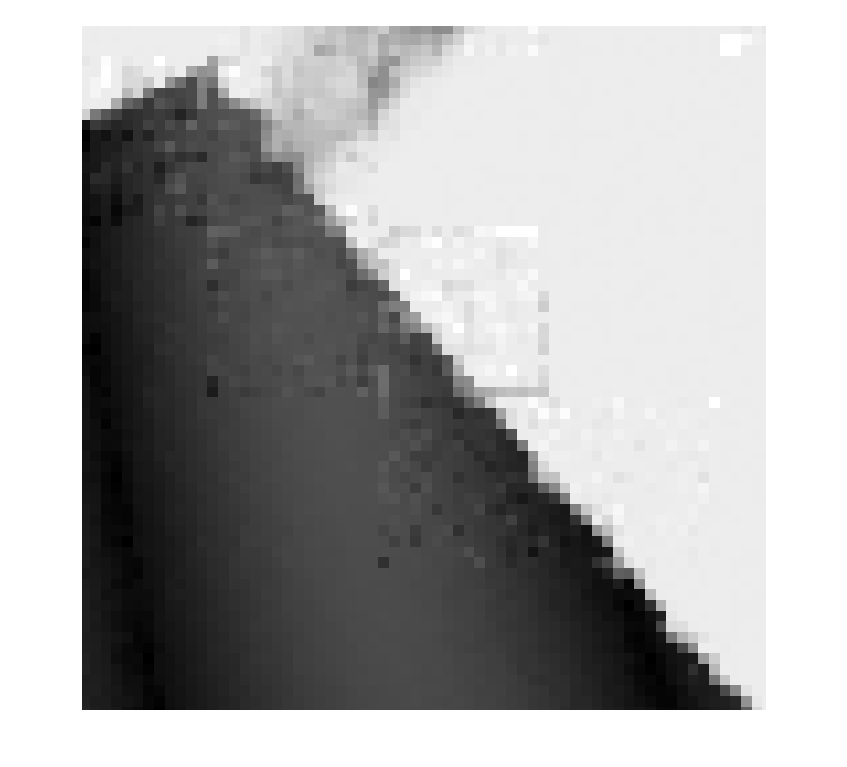
\includegraphics[width=\columnwidth]{images/boundaryArtifact_noframe.png}
  \caption{Artifacts that occur without a frame (frame size = 0). The patches are recognizable in the reconstruction}
  \label{fig:boundaryArtifacts}
\end{figure}

\begin{figure}[tbp]
  \centering
  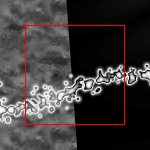
\includegraphics[width=\columnwidth]{images/imageFraming.png}
  \caption{Only the inner patch (marked red) is reconstructed in one step while the frame only provides additional signal. (Undistorted image shown) }
  \label{fig:framing}
\end{figure}

((( TODO: Insert plot MissingPixels vs. Accuracy )))

Use examples and illustrations to clarify ideas and results. For
example, by comparing Figure~\ref{fig:framing} and
Figure~\ref{fig:flowchart}, we can see the two different
situations where Fourier and wavelet basis perform well. 

\section{Summary}
(((( TODO ))))
  Summarise your contributions in light of the new
  results.
  

\section*{Acknowledgements}
We would like to recognize and thank the following individuals or groups for their contribution to this work:\\
Our implementation is based on the inpainting and evaluation framework provided by the course "Computer Intelligence Lab" held by Prof. Joachim Buhmann at ETH Zürich.
(((( TODO ))))


\bibliographystyle{IEEEtran}
\bibliography{biblio}


\begin{figure*}[b]
  \centering
  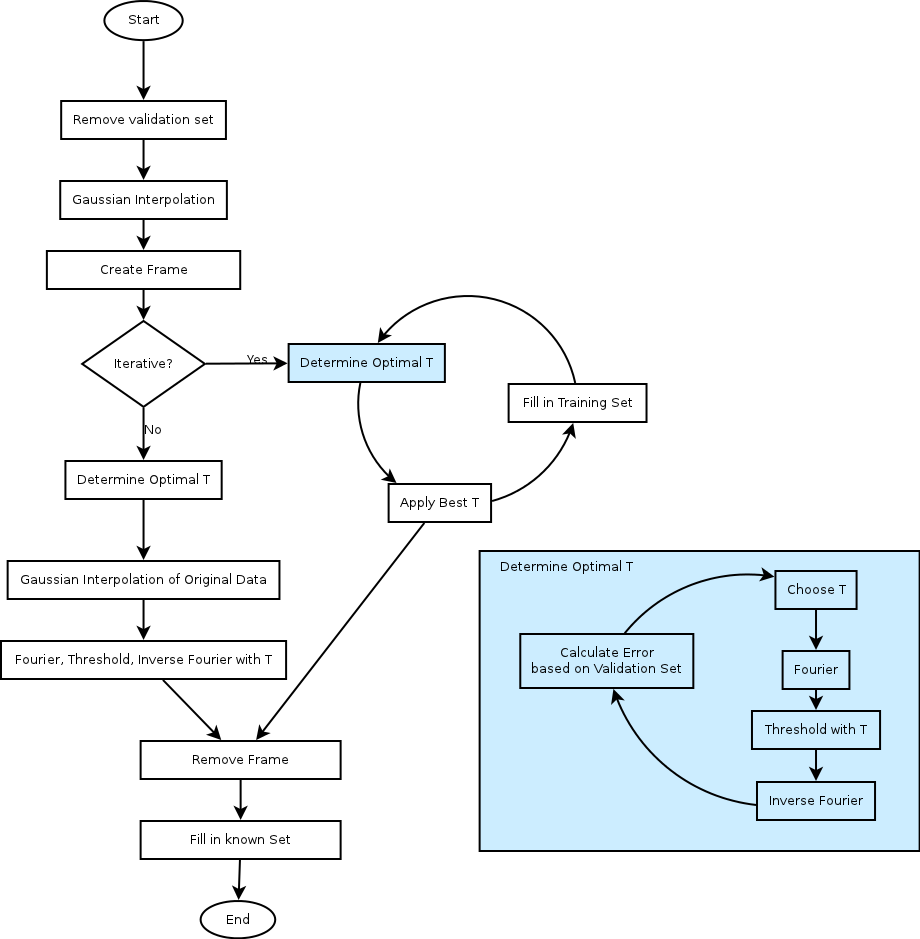
\includegraphics[width= 400px]{images/flowchart}
  \caption{The algorithm as a flow chart}
  \label{fig:flowchart}
\end{figure*}
\end{document}
